% network.tex
%
% Network subsection of the Running main section.

%begin{latexonly}
  \newcommand{\modgraphic}%
  {\centerline{\epsfig{file=figures/modgraphic.eps,width=\columnwidth}}}
%end{latexonly}
\begin{htmlonly}
  \newcommand{\srwindow}{%
  \htmladdimg[align=top,width=6,alt="SCIRun Window"]
  {../figures/modgraphic.gif}}
\end{htmlonly}

\section{Working with Networks}
\label{sec:workwithnets}

This section describes how to create, save, open, execute, and edit
networks.

Starting \sr\ (with no arguments) will create the \sr\ main window with a
blank network pane window.  The goal then is to build a network by
creating and connecting modules.


\subsection{Creating a Module}
\label{sec:creatingmodules}

Create a module by selecting its name from one of the package (\eg \sr)
menu's category submenu.  The package menus may be accessed from the main
window's menu bar and from the network pane's popup menu.

Activate the network pane's popup menu by clicking the right most mouse
button while the mouse pointer is in the network pane.  The popup menu
contains a list of category submenus from the \sr package and any
additional packages.  And of course each category submenu provides access
to the modules within the category.

After creating a module its graphic ``front end'' will be created and
placed in the network pane.

\subsubsection{Anatomy of a Module}
\label{sec:modanatomy}

All modules are represented similarly by a graphic within the network pane.
See Figure~\ref{fig:modgraphic}. For all modules this graphical ``front
end'' consists of the following components:

\begin{description}
\item[Name] The module's name.
\item[Input ports] Zero or more input ports.  Each port corresponds to a
  data type and each data type has a unique color.
  Table~\ref{tab:portcolors} maps port colors to data types.  Input ports
  connect to other modules' output ports.
\item[Output ports] Zero or more output ports.  Output ports connect to
  other modules' input ports.  Every module has, of course, at least 1 input
  or 1 output port.
\item[UI button] Pressing the \button{UI} button displays the module's
  control dialog. Some modules have no such dialog. Some have very
  simple dialogs.  Some have very complex dialogs which allow elaborate
  control over the module.  
\item[Progress bar] Shows the module's progress.
\item[Timer] Displays the amount of CPU time the module has consumed.
\item[Popup Menu] Pressing the right most mouse button while the mouse
  pointer is over a module gives access to the module's popup menu.  The
  popup menu gives access to the following items:
  \begin{description}
  \item[::Package_Category_Name_Instance]  This is item is just a label.
    It tells you the name of the module and the category and package the
    module belongs to.  The Instance part is a unique number which
    distinguishes multiple module instances of the same type.
  \item[Execute] Executes the network.
  \item[Notes] This item displays the module's note pad.  Use the note pad
    to document the purpose of the module in the current network.
  \item[Destroy] Destroys the module.
  \item[Show Log] Displays the module's message log.  Most modules will
    write messages to the log during the course of their execution.
  \item[Show Status] This item is a toggle button which turns off/on the
    display of the progress indicator.  Turning off the progress indicator
    can help speed up the execution of complex networks.
  \end{description}
\end{description}

\begin{table}[htbp]
  \begin{center}
    \begin{tabular}{|l|l|}
      \textbf{Data Type} & \textbf{Port Color} \\
      \hline
      Field & Yellow \\
      Field Set & Green \\
      Matricies & Blue \\
      Geometric Objects & Pink \\
      Color Maps & Purple \\
      Camera Path & Brown \\
      \hline
    \end{tabular}
    \caption{Data Types and their Port Colors}
    \label{tab:portcolors}
  \end{center}
\end{table}


\begin{figure}[htb]
  \begin{makeimage}
  \end{makeimage}
  \modgraphic
%  \centerline{\epsfig{file=figures/modgraphic.eps,width=6in}}
  \caption{\label{fig:module} \sr\ module}
\end{figure}


\subsection{Connecting Modules}
\label{sec:connectmods}



\subsection{Moving  Module}
\label{sec:movemod}


\subsection{Setting a Module's Properties}
\label{sec:setmodprops}


\subsection{Executing a Network}
\label{sec:executenet}


\subsection{Deleting a Connection}
\label{sec:deleteconnections}


\subsection{Deleting a Module}
\label{sec:deletemod}


\subsection{Documenting a Module}
\label{sec:docmodule}


\subsection{Viewing a Module's Log}
\label{sec:viewmodslog}


\subsection{Documenting a Network}
\label{sec:docnetwork}


\subsection{Saving a Network}
\label{sec:savenet}


\subsection{Opening a Network}
\label{sec:opennet}


%%% Local Variables: 
%%% mode: latex
%%% TeX-master: "usersguide"
%%% End: 
